\documentclass[12pt,letterpaper]{article}
\usepackage{graphicx,textcomp}
\usepackage{natbib}
\usepackage{setspace}
\usepackage{fullpage}
\usepackage{color}
\usepackage[reqno]{amsmath}
\usepackage{amsthm}
\usepackage{fancyvrb}
\usepackage{amssymb,enumerate}
\usepackage[all]{xy}
\usepackage{endnotes}
\usepackage{lscape}
\newtheorem{com}{Comment}
\usepackage{float}
\usepackage{hyperref}
\newtheorem{lem} {Lemma}
\newtheorem{prop}{Proposition}
\newtheorem{thm}{Theorem}
\newtheorem{defn}{Definition}
\newtheorem{cor}{Corollary}
\newtheorem{obs}{Observation}
\usepackage[compact]{titlesec}
\usepackage{dcolumn}
\usepackage{tikz}
\usetikzlibrary{arrows}
\usepackage{multirow}
\usepackage{xcolor}
\newcolumntype{.}{D{.}{.}{-1}}
\newcolumntype{d}[1]{D{.}{.}{#1}}
\definecolor{light-gray}{gray}{0.65}
\usepackage{url}
\usepackage{listings}
\usepackage{color}

\definecolor{codegreen}{rgb}{0,0.6,0}
\definecolor{codegray}{rgb}{0.5,0.5,0.5}
\definecolor{codepurple}{rgb}{0.58,0,0.82}
\definecolor{backcolour}{rgb}{0.95,0.95,0.92}

\lstdefinestyle{mystyle}{
	backgroundcolor=\color{backcolour},   
	commentstyle=\color{codegreen},
	keywordstyle=\color{magenta},
	numberstyle=\tiny\color{codegray},
	stringstyle=\color{codepurple},
	basicstyle=\footnotesize,
	breakatwhitespace=false,         
	breaklines=true,                 
	captionpos=b,                    
	keepspaces=true,                 
	numbers=left,                    
	numbersep=5pt,                  
	showspaces=false,                
	showstringspaces=false,
	showtabs=false,                  
	tabsize=2
}
\lstset{style=mystyle}
\newcommand{\Sref}[1]{Section~\ref{#1}}
\newtheorem{hyp}{Hypothesis}

\title{Problem Set 3}
\date{Due: November 19, 2023}
\author{Student: Shekhar Kedia (23351315)\\
	Applied Stats/Quant Methods 1}

\begin{document}
	\maketitle
	\section*{Instructions}
	\begin{itemize}
		\item Please show your work! You may lose points by simply writing in the answer. If the problem requires you to execute commands in \texttt{R}, please include the code you used to get your answers. Please also include the \texttt{.R} file that contains your code. If you are not sure if work needs to be shown for a particular problem, please ask.
	\item Your homework should be submitted electronically on GitHub.
	\item This problem set is due before 23:59 on Sunday November 19, 2023. No late assignments will be accepted.

	\end{itemize}

		\vspace{.25cm}
	
\noindent In this problem set, you will run several regressions and create an add variable plot (see the lecture slides) in \texttt{R} using the \texttt{incumbents\_subset.csv} dataset. Include all of your code.\\

\textbf{\texttt{R} code to read the dataset:}
\lstinputlisting[language=R, firstline=35, lastline=36]{PS3_Shekhar Kedia.R}  

	\vspace{.5cm}
\pagebreak
\section*{Question 1}
\vspace{.25cm}
\noindent We are interested in knowing how the difference in campaign spending between incumbent and challenger affects the incumbent's vote share. 
	\begin{enumerate}
		\item Run a regression where the outcome variable is \texttt{voteshare} and the explanatory variable is \texttt{difflog}.
		
		\textbf{\texttt{R} code to run the regression and create the output:}
		\lstinputlisting[language=R, firstline=39, lastline=44]{PS3_Shekhar Kedia.R}  
		
		\begin{table}[!htbp] \centering 
			\caption{Model 1 Regression Results} 
			\label{} 
			\begin{tabular}{@{\extracolsep{5pt}}lc} 
				\\[-1.8ex]\hline 
				\hline \\[-1.8ex] 
				& \multicolumn{1}{c}{\textit{Dependent variable:}} \\ 
				\cline{2-2} 
				\\[-1.8ex] & voteshare \\ 
				\hline \\[-1.8ex] 
				difflog & 0.042$^{***}$ \\ 
				& (0.001) \\ 
				& \\ 
				Constant & 0.579$^{***}$ \\ 
				& (0.002) \\ 
				& \\ 
				\hline \\[-1.8ex] 
				Observations & 3,193 \\ 
				R$^{2}$ & 0.367 \\ 
				Adjusted R$^{2}$ & 0.367 \\ 
				Residual Std. Error & 0.079 (df = 3191) \\ 
				F Statistic & 1,852.791$^{***}$ (df = 1; 3191) \\ 
				\hline 
				\hline \\[-1.8ex] 
				\textit{Note:}  & \multicolumn{1}{r}{$^{*}$p$<$0.1; $^{**}$p$<$0.05; $^{***}$p$<$0.01} \\ 
			\end{tabular} 
		\end{table} 
		
		\textbf{Interpretation:}\\
		The above model shows that one unit increase in log difference in campaign spending between incumbent and challenger is associated with, on average, a 0.042 unit increase in incumbent's vote share.

\pagebreak

		\item Make a scatterplot of the two variables and add the regression line. 	
		
		\textbf{\texttt{R} code to create the scatter plot and add the regression line:}
		\lstinputlisting[language=R, firstline=47, lastline=54]{PS3_Shekhar Kedia.R}  
		
		\begin{center}
			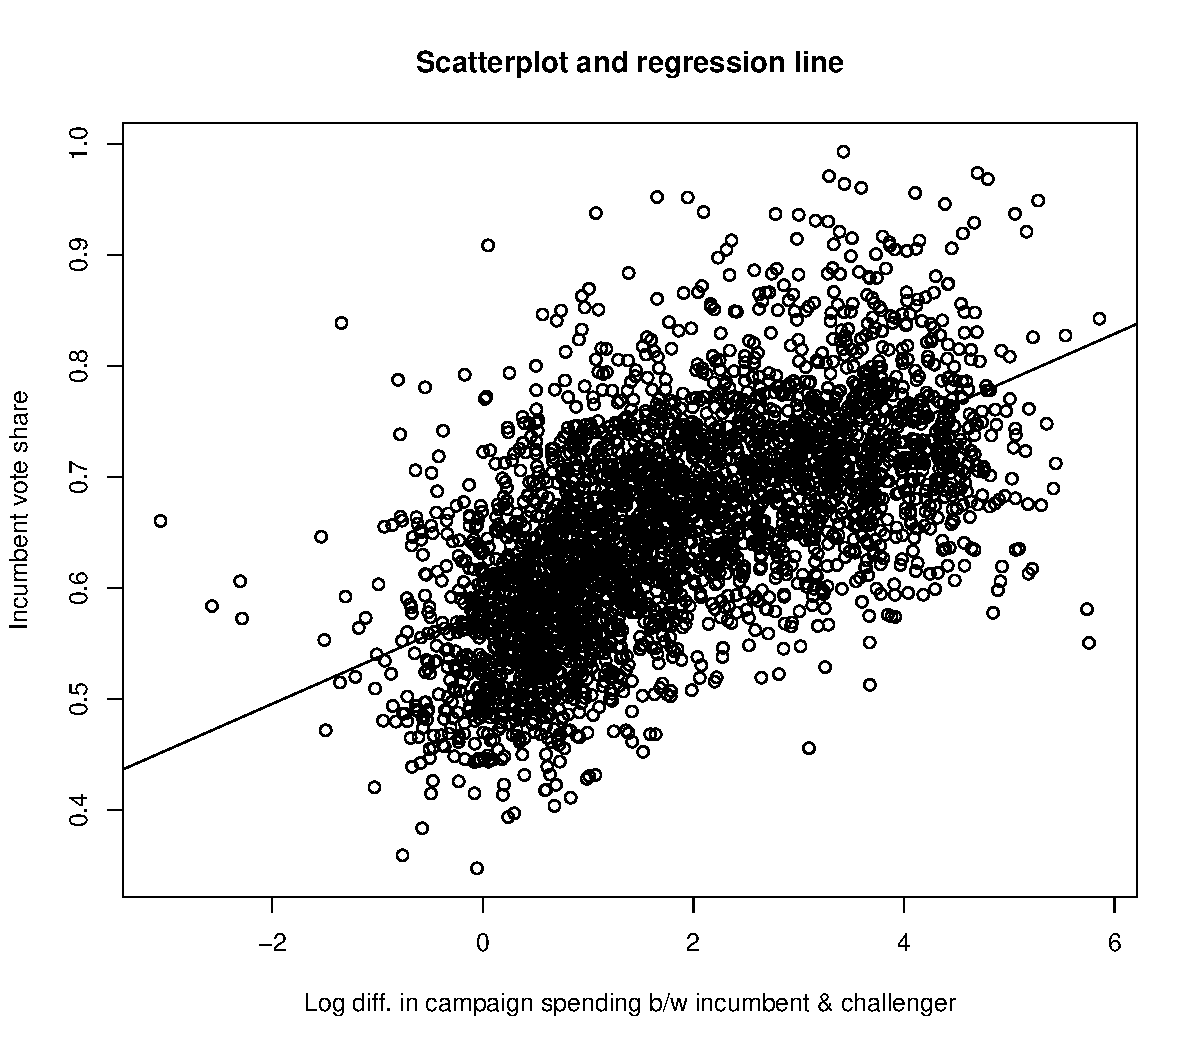
\includegraphics[width=15cm]{plot1.pdf}  
		\end{center}
		
		\item Save the residuals of the model in a separate object.
		
		\textbf{\texttt{R} code to save the residuals of the model in a separate object:}
		\lstinputlisting[language=R, firstline=57, lastline=57]{PS3_Shekhar Kedia.R}
		
		\item Write the prediction equation.
		
		\noindent The general form for bivariate equation is:
		$\hat{Y} = b_0 + b_1 X_1$\\
		\\Where,\\
		$\hat{Y}$ is the predicted value of the outcome variable,\\
		$b_0$ is the y-intercept (the value of $\hat{Y}$ when $X_1$ is 0),\\
		$b_1$ is the slope of the regression line, representing the change in $\hat{Y}$ for a one-unit change in $X_1$,\\
		$X_1$ is the explanatory variable\\
		\\
		In the context of the model, the predicted equation is:\\
		\textit{$\texttt{voteshare} = 0.579 + 0.042*\texttt{difflog}$}

	\end{enumerate}
	\vspace*{1cm}
\section*{Question 2}
\noindent We are interested in knowing how the difference between incumbent and challenger's spending and the vote share of the presidential candidate of the incumbent's party are related.	\vspace{.25cm}
	\begin{enumerate}
		\item Run a regression where the outcome variable is \texttt{presvote} and the explanatory variable is \texttt{difflog}.
		
		\vspace{.25cm}
		
		\textbf{\texttt{R} code to run the regression and create the output:}
		\lstinputlisting[language=R, firstline=64, lastline=69]{PS3_Shekhar Kedia.R}  
		
		\begin{table}[!htbp] \centering 
			\caption{Model 2 Regression Results} 
			\label{} 
			\begin{tabular}{@{\extracolsep{5pt}}lc} 
				\\[-1.8ex]\hline 
				\hline \\[-1.8ex] 
				& \multicolumn{1}{c}{\textit{Dependent variable:}} \\ 
				\cline{2-2} 
				\\[-1.8ex] & presvote \\ 
				\hline \\[-1.8ex] 
				difflog & 0.024$^{***}$ \\ 
				& (0.001) \\ 
				& \\ 
				Constant & 0.508$^{***}$ \\ 
				& (0.003) \\ 
				& \\ 
				\hline \\[-1.8ex] 
				Observations & 3,193 \\ 
				R$^{2}$ & 0.088 \\ 
				Adjusted R$^{2}$ & 0.088 \\ 
				Residual Std. Error & 0.110 (df = 3191) \\ 
				F Statistic & 307.715$^{***}$ (df = 1; 3191) \\ 
				\hline 
				\hline \\[-1.8ex] 
				\textit{Note:}  & \multicolumn{1}{r}{$^{*}$p$<$0.1; $^{**}$p$<$0.05; $^{***}$p$<$0.01} \\ 
			\end{tabular} 
		\end{table} 
		
		\pagebreak
		
		\textbf{Interpretation:}\\
		The above model shows that one unit increase in log difference in campaign spending between incumbent and challenger is associated with, on average, a 0.024 unit increase in vote share of the presidential candidate of the incumbent's party.\\
		
		\item Make a scatterplot of the two variables and add the regression line.\\
		
		\textbf{\texttt{R} code to create the scatter plot and add the regression line:}
		\lstinputlisting[language=R, firstline=72, lastline=79]{PS3_Shekhar Kedia.R}  
		
		\begin{center}
			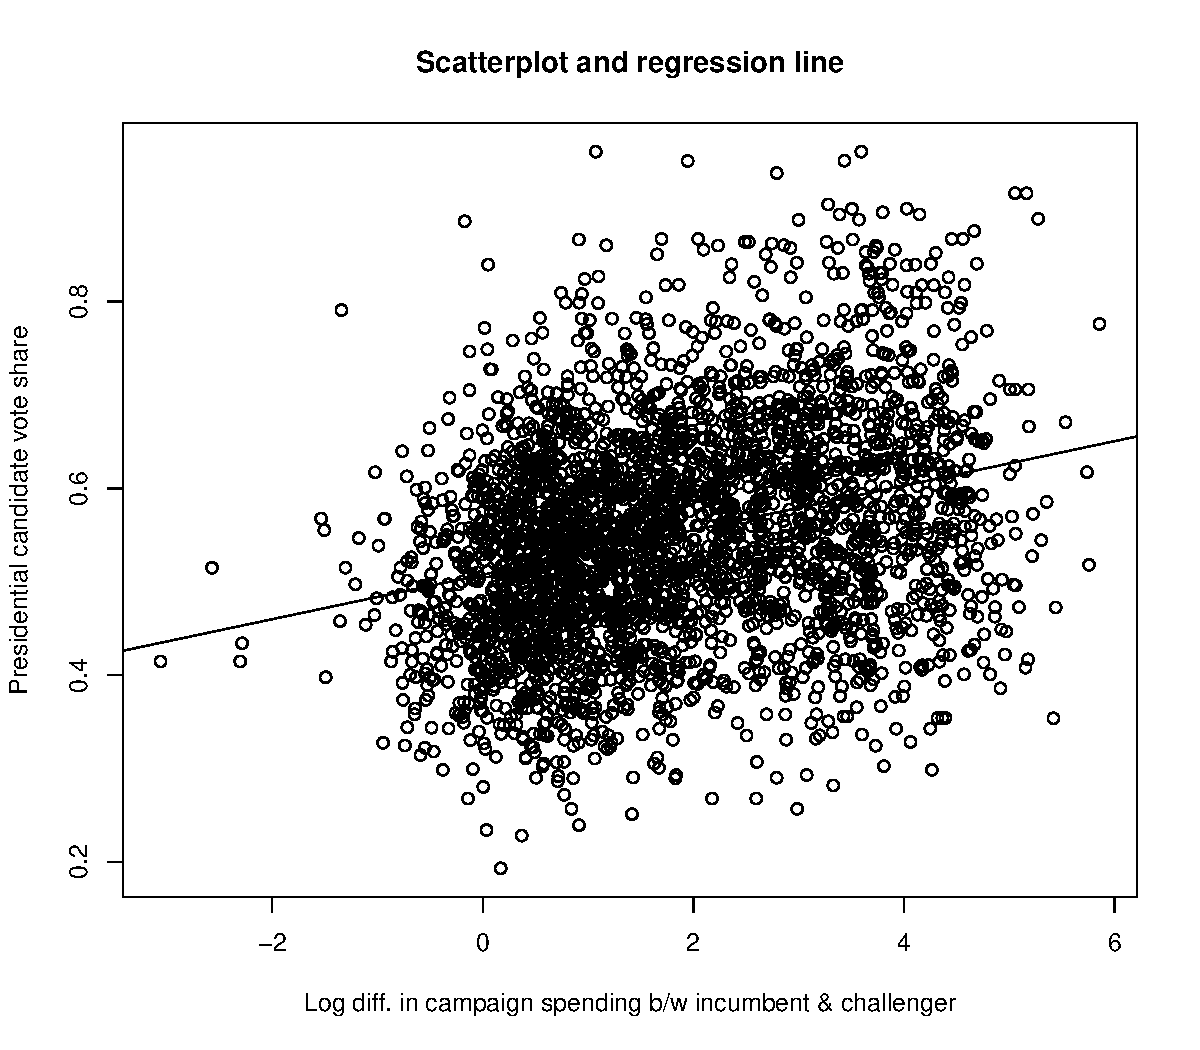
\includegraphics[width=14cm]{plot2.pdf}  
		\end{center}
		
		\item Save the residuals of the model in a separate object.
		
		\textbf{\texttt{R} code to save the residuals of the model in a separate object:}
		\lstinputlisting[language=R, firstline=82, lastline=82]{PS3_Shekhar Kedia.R}  
		
		\item Write the prediction equation.
		
		\noindent The general form for bivariate equation is:
		$\hat{Y} = b_0 + b_1 X_1$\\
		\\Where,\\
		$\hat{Y}$ is the predicted value of the outcome variable,\\
		$b_0$ is the y-intercept (the value of $\hat{Y}$ when $X_1$ is 0),\\
		$b_1$ is the slope of the regression line, representing the change in $\hat{Y}$ for a one-unit change in $X_1$,\\
		$X_1$ is the explanatory variable\\
		\\
		In the context of the model, the predicted equation is:\\
		\textit{$\texttt{presvote} = 0.508 + 0.024*\texttt{difflog}$}
		
	\end{enumerate}
	
	\newpage	
\section*{Question 3}

\noindent We are interested in knowing how the vote share of the presidential candidate of the incumbent's party is associated with the incumbent's electoral success.
	\vspace{.25cm}
	\begin{enumerate}
		\item Run a regression where the outcome variable is \texttt{voteshare} and the explanatory variable is \texttt{presvote}.
		
		\textbf{\texttt{R} code to run the regression and create the output:}
		\lstinputlisting[language=R, firstline=89, lastline=94]{PS3_Shekhar Kedia.R}
		
		\begin{table}[!htbp] \centering 
			\caption{Model 3 Regression Results} 
			\label{} 
			\begin{tabular}{@{\extracolsep{5pt}}lc} 
				\\[-1.8ex]\hline 
				\hline \\[-1.8ex] 
				& \multicolumn{1}{c}{\textit{Dependent variable:}} \\ 
				\cline{2-2} 
				\\[-1.8ex] & voteshare \\ 
				\hline \\[-1.8ex] 
				presvote & 0.388$^{***}$ \\ 
				& (0.013) \\ 
				& \\ 
				Constant & 0.441$^{***}$ \\ 
				& (0.008) \\ 
				& \\ 
				\hline \\[-1.8ex] 
				Observations & 3,193 \\ 
				R$^{2}$ & 0.206 \\ 
				Adjusted R$^{2}$ & 0.206 \\ 
				Residual Std. Error & 0.088 (df = 3191) \\ 
				F Statistic & 826.950$^{***}$ (df = 1; 3191) \\ 
				\hline 
				\hline \\[-1.8ex] 
				\textit{Note:}  & \multicolumn{1}{r}{$^{*}$p$<$0.1; $^{**}$p$<$0.05; $^{***}$p$<$0.01} \\ 
			\end{tabular} 
		\end{table} 
		
		\textbf{Interpretation:}\\
		The above model shows that one unit increase in the vote share of the presidential candidate of the incumbent's party is associated with, on average, a 0.388 unit increase in incumbent's vote share.

		\item Make a scatterplot of the two variables and add the regression line. 
		
		\textbf{\texttt{R} code to create the scatter plot and add the regression line:}
		\lstinputlisting[language=R, firstline=97, lastline=104]{PS3_Shekhar Kedia.R}  
		
		\begin{center}
			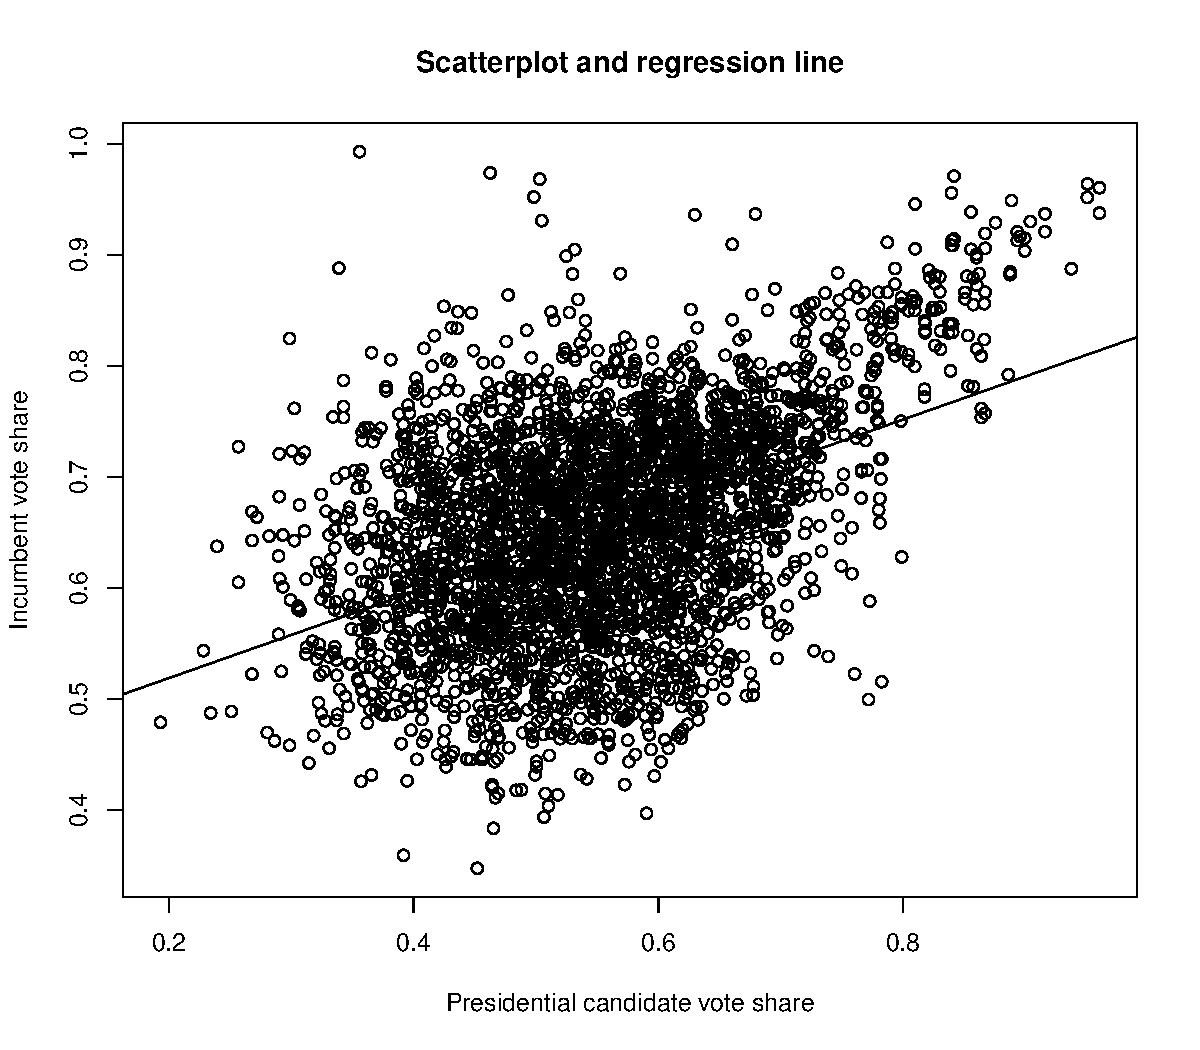
\includegraphics[width=14cm]{plot3.pdf}  
		\end{center}

		\item Write the prediction equation.
		\noindent The general form for bivariate equation is:
		$\hat{Y} = b_0 + b_1 X_1$\\
		\\Where,\\
		$\hat{Y}$ is the predicted value of the outcome variable,\\
		$b_0$ is the y-intercept (the value of $\hat{Y}$ when $X_1$ is 0),\\
		$b_1$ is the slope of the regression line, representing the change in $\hat{Y}$ for a one-unit change in $X_1$,\\
		$X_1$ is the explanatory variable\\
		\\
		In the context of the model, the predicted equation is:\\
		\textit{$\texttt{voteshare} = 0.441 + 0.388*\texttt{presvote}$}

	\end{enumerate}
	

\newpage	
\section*{Question 4}
\noindent The residuals from part (a) tell us how much of the variation in \texttt{voteshare} is $not$ explained by the difference in spending between incumbent and challenger. The residuals in part (b) tell us how much of the variation in \texttt{presvote} is $not$ explained by the difference in spending between incumbent and challenger in the district.
	\begin{enumerate}
		\item Run a regression where the outcome variable is the residuals from Question 1 and the explanatory variable is the residuals from Question 2.
		
		\textbf{\texttt{R} code to run the regression and create the output:}
		\lstinputlisting[language=R, firstline=110, lastline=115]{PS3_Shekhar Kedia.R}
		
		\begin{table}[!htbp] \centering 
			\caption{Model 4 Regression Results} 
			\label{} 
			\begin{tabular}{@{\extracolsep{5pt}}lc} 
				\\[-1.8ex]\hline 
				\hline \\[-1.8ex] 
				& \multicolumn{1}{c}{\textit{Dependent variable:}} \\ 
				\cline{2-2} 
				\\[-1.8ex] & residuals\_vote\_diff \\ 
				\hline \\[-1.8ex] 
				residuals\_pres\_diff & 0.257$^{***}$ \\ 
				& (0.012) \\ 
				& \\ 
				Constant & $-$0.000 \\ 
				& (0.001) \\ 
				& \\ 
				\hline \\[-1.8ex] 
				Observations & 3,193 \\ 
				R$^{2}$ & 0.130 \\ 
				Adjusted R$^{2}$ & 0.130 \\ 
				Residual Std. Error & 0.073 (df = 3191) \\ 
				F Statistic & 476.975$^{***}$ (df = 1; 3191) \\ 
				\hline 
				\hline \\[-1.8ex] 
				\textit{Note:}  & \multicolumn{1}{r}{$^{*}$p$<$0.1; $^{**}$p$<$0.05; $^{***}$p$<$0.01} \\ 
			\end{tabular} 
		\end{table}
		
		\textbf{Interpretation:}\\
		The above model shows that one unit increase in residuals from Question 2 (i.e, unexplained variation in \texttt{presvote} by the log difference in spending between incumbent and challenger) is associated with, on average, a 0.257 unit increase in residuals from Question 1 (i.e, unexplained variation in \texttt{voteshare} by the log difference in spending between incumbent and challenger).\\
		
		\item Make a scatterplot of the two residuals and add the regression line.
		
		\textbf{\texttt{R} code to create the scatter plot and add the regression line:}
		\lstinputlisting[language=R, firstline=118, lastline=125]{PS3_Shekhar Kedia.R}  
		
		\begin{center}
			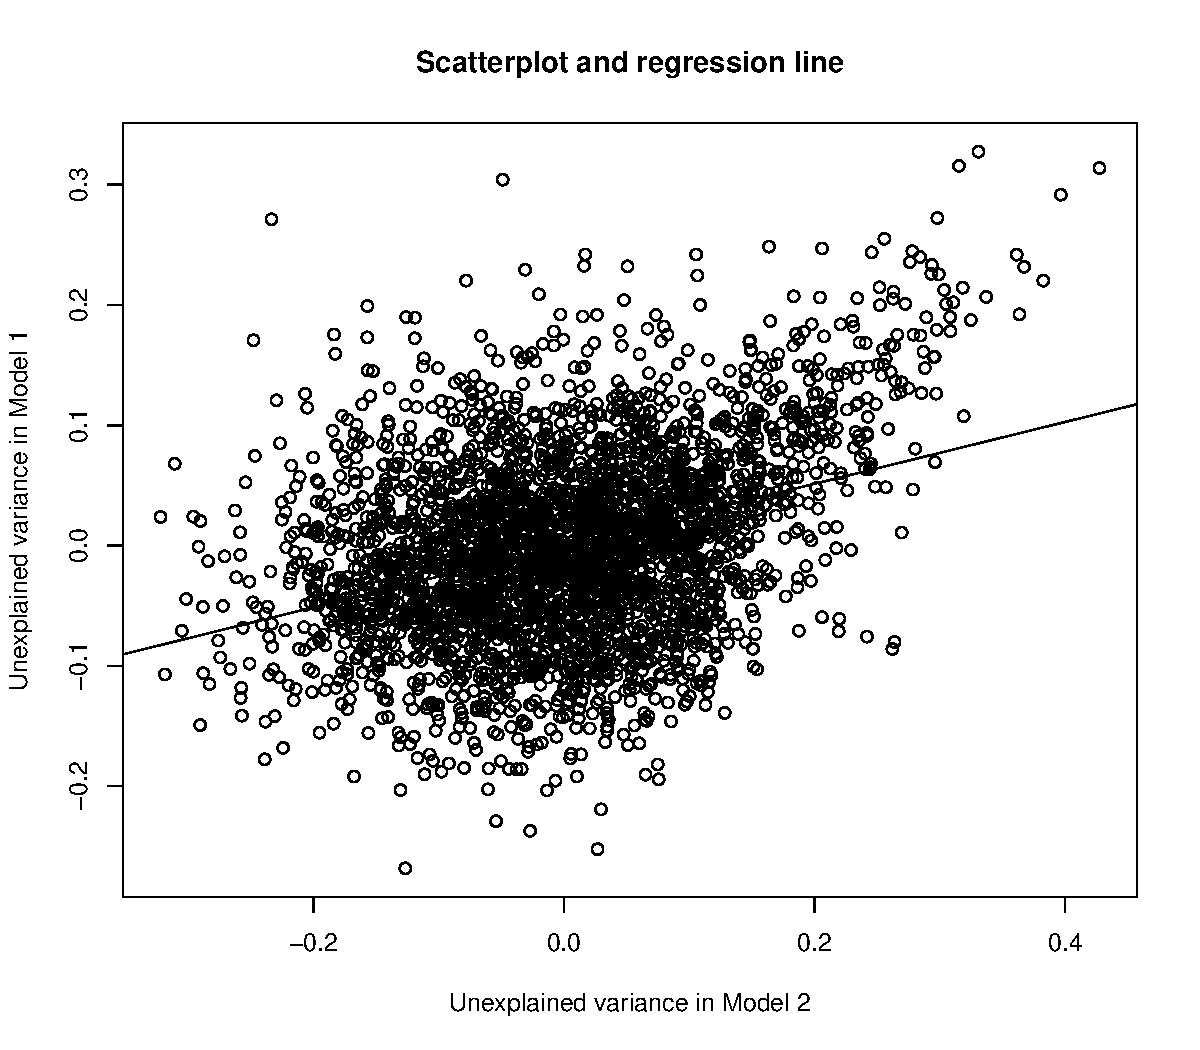
\includegraphics[width=15cm]{plot4.pdf}  
		\end{center}
		
		\pagebreak
		
		\item Write the prediction equation.
		
		\noindent The general form for bivariate equation is:
		$\hat{Y} = b_0 + b_1 X_1$\\
		\\Where,\\
		$\hat{Y}$ is the predicted value of the outcome variable,\\
		$b_0$ is the y-intercept (the value of $\hat{Y}$ when $X_1$ is 0),\\
		$b_1$ is the slope of the regression line, representing the change in $\hat{Y}$ for a one-unit change in $X_1$,\\
		$X_1$ is the explanatory variable\\
		\\
		In the context of the model, the predicted equation is:\\
		\textit{$\texttt{residuals\_vote\_diff} = -5.934e^{-18} + 0.257*\texttt{residuals\_pres\_diff}$}
		
	\end{enumerate}
	
	\vspace*{1cm}


\section*{Question 5}
\noindent What if the incumbent's vote share is affected by both the president's popularity and the difference in spending between incumbent and challenger? 
\vspace*{0.5cm}
	\begin{enumerate}
		\item Run a regression where the outcome variable is the incumbent's \texttt{voteshare} and the explanatory variables are \texttt{difflog} and \texttt{presvote}.\\
		
		\textbf{\texttt{R} code to run the regression and create the output:}
		\lstinputlisting[language=R, firstline=131, lastline=136]{PS3_Shekhar Kedia.R}
		
		\begin{table}[!htbp] \centering 
			\caption{Model 5 Regression Results} 
			\label{} 
			\begin{tabular}{@{\extracolsep{5pt}}lc} 
				\\[-1.8ex]\hline 
				\hline \\[-1.8ex] 
				& \multicolumn{1}{c}{\textit{Dependent variable:}} \\ 
				\cline{2-2} 
				\\[-1.8ex] & voteshare \\ 
				\hline \\[-1.8ex] 
				difflog & 0.036$^{***}$ \\ 
				& (0.001) \\ 
				& \\ 
				presvote & 0.257$^{***}$ \\ 
				& (0.012) \\ 
				& \\ 
				Constant & 0.449$^{***}$ \\ 
				& (0.006) \\ 
				& \\ 
				\hline \\[-1.8ex] 
				Observations & 3,193 \\ 
				R$^{2}$ & 0.450 \\ 
				Adjusted R$^{2}$ & 0.449 \\ 
				Residual Std. Error & 0.073 (df = 3190) \\ 
				F Statistic & 1,302.947$^{***}$ (df = 2; 3190) \\ 
				\hline 
				\hline \\[-1.8ex] 
				\textit{Note:}  & \multicolumn{1}{r}{$^{*}$p$<$0.1; $^{**}$p$<$0.05; $^{***}$p$<$0.01} \\ 
			\end{tabular} 
		\end{table}

		\pagebreak
		
		\textbf{Interpretation:}\\
		The above model shows that holding the president's popularity constant, one unit increase in log difference in spending between incumbent and challenger is associated with, on average, a 0.036 unit increase in incumbent's vote share.\\
		Furthermore, the model shows that holding the log difference in spending between incumbent and challenger constant, one unit increase in president's popularity is associated with, on average, a 0.257 unit increase in incumbent's vote share.
				
		\item Write the prediction equation.
		
		\noindent The general form for multivariate equation is:
		$\hat{Y} = b_0 + b_1 X_1 + b_2 X_2 + .... + b_n X_n$\\
		\\Where,\\
		$\hat{Y}$ is the predicted value of the outcome variable,\\
		$b_0$ is the y-intercept (the value of $\hat{Y}$ when $X_1, X_2, ..., X_n$ are 0),\\
		$b_1, b_2, ..., b_n$ are the slopes of the regression model, representing the change in $\hat{Y}$ for a one-unit change in $X_1, X_2, ..., X_n$ respectively keeping all other values constant,\\
		$X_1, X_2, ..., X_n$ are the explanatory variables\\
		\\
		In the context of the model, the predicted equation is:\\
		\textit{$\texttt{voteshare} = 0.448 + 0.0355*\texttt{difflog} + 0.256*\texttt{presvote}$}
		
		\item What is it in this output that is identical to the output in Question 4? Why do you think this is the case?
		
		The coefficient of \texttt{presvote} in the model from Question 5 is identical to the coefficient of residuals from Question 2 (i.e, unexplained variation in \texttt{presvote} by the log difference in spending between incumbent and challenger) in the model from Question 4, i.e., 0.257.\\
		
		
		Looking at the regression model for Question 4, we understand how much the residuals of Question 2 contribute to explaining the variance in the residuals of Question 1.\\
		Now, the regression model for Question 5 includes both \texttt{presvote} and log difference in spending between incumbent and challenger as predictor for incumbent's vote share.
		Here, the coefficient of \texttt{presvote} in Question 5 represents the partial impact of \texttt{presvote} on incumbent's vote share, accounting for the relationship between \texttt{presvote} and the residuals of Question 1 which is similar to Question 4.
		
		
		
	\end{enumerate}




\end{document}
